\chapter{Methods}
\label{chap:methods}

As discussed in \autoref{chap:introduction}, the system developed in this thesis follows a pipeline consisting of two steps:
\begin{enumerate}
    \item \textbf{Object Proposal}: detection of all the logos in the image
    \item \textbf{Classification}: recognize each logo
\end{enumerate}
The first step regarding the detection of logos in the image is done by YOLO (see \autoref{sec:yolo}), while the actual recognition of the logo is performed by the classifier in an incremental learning setup. The pipeline of the system is shown in \autoref{fig:roi_and_classification}.

\begin{figure}%
	\centering

    \begin{center}
        \includegraphics[width=\columnwidth]{images/roi+classification.drawio.png}
    \end{center}

	\caption{Pipeline of the system: the class-agnostic logo detector generates ROIs, then the classification is performed by the CIL classifier.}%
	\label{fig:roi_and_classification}%
\end{figure}

The detector used in the first step is a class-agnostic logo detector: it is a logo detector since we are not interested in the detection of objects other than logo; and it is class-agnostic since the number of detected classes is only one. In fact, in this first step the detector will be responsible for finding any generic logo (i.e., a single class) in the image. This is a crucial step if we seek to achieve incremental learning logo recognition, because in this way it is possible to decouple the detection from the recognition. If the logo detector localize any generic logo in the image, and delegates the actual recognition to the CIL classifier, there is no need to develop an incremental learning detector as well.


An important aspect of the classifier is the model size in terms of number of parameters. A big model comes with several disadvantages like longer time for the training phase, higher memory requirements and longer time to make inference. To this reason, a part of this work aims to decrease the number of parameters of the classifier using two different techniques. The first technique is described in \autoref{sec:method-pruning}, using masking and pruning described in \autoref{sec:masking-pruning} it aims to prune the model after the training of each incremental step, thus reducing the number of parameters. The second approach is the Knowledge Distillation (KD) described in \autoref{sec:method-kd}, where a smaller model is trained from scratch with the supervision of a bigger model trained on the same task.


\vspace{1.5\baselineskip}
This chapter describes all the details about the logo detector in \autoref{sec:method-roi} and continues with the classifier in \autoref{sec:method-classifier}. Then, in \autoref{sec:method-pruning} and \autoref{sec:method-kd} are discussed some techniques with the purpose to reducing the number of parameters of the model. In order to evaluate the drop in the terms of performance of the CIL classifier when compared to a standard close-set classification task (i.e. all the classes are available ath the beginning and there is no need to introduce new classes during time),
the chapter ends in \autoref{sec:method-baseline} with the introduction of different baselines.

The code develop during this thesis is available in the GitHub repository \footnote{GitHub repository relative to the code of developed in this thesis: \\ \href{https://github.com/gianlucagiudice/logo-detection-recognition}{https://github.com/gianlucagiudice/logo-detection-recognition}} linked below.


\section{Region proposal}
A key component of the system is the logo detector. Formally, this first step is an object detection task, where the objects we seek to detect are the logos in the image. The logo detector produces in output the coordinates of the bounding boxes corresponding to the logos in the image. The bounding boxes can be used to crop the portions of the images generating the regions of interest (ROIs). The ROIs corresponds to what the detector considers as any generic logo, and these can be directly used as input for the CIL model which classifies (i.e. recognize) the logo.


\label{sec:method-roi}
\subsection{YOLOv5m6}
The class-agnostic logo detector is based on YOLOv5-v6.0 \cite{glenn_jocher_2021_5563715}. There are different versions of YOLOv5-v6.0, depending on the size of the model (in terms of the number of parameters), and the size of the input image. In general, larger models perform better, with the disadvantage of longer training time, longer inference time and more computational resources required to train the model. On the other hand, a small model might achieve very low performance, thus misleading the final evaluation of the system, which is actually caused by the small model acting as a bottleneck. On the other hand, a small model might achieve very low performance, thus misleading the final evaluation of the system that relies heavily on the detector. Therefore, a model that is too small could act as a bottleneck for the whole system. A more detailed analysis on the tradeoff is shown in \autoref{fig:yolo-sizes} and \autoref{table:yolo-sizes}.

\begin{figure}%
	\centering

    \begin{center}
        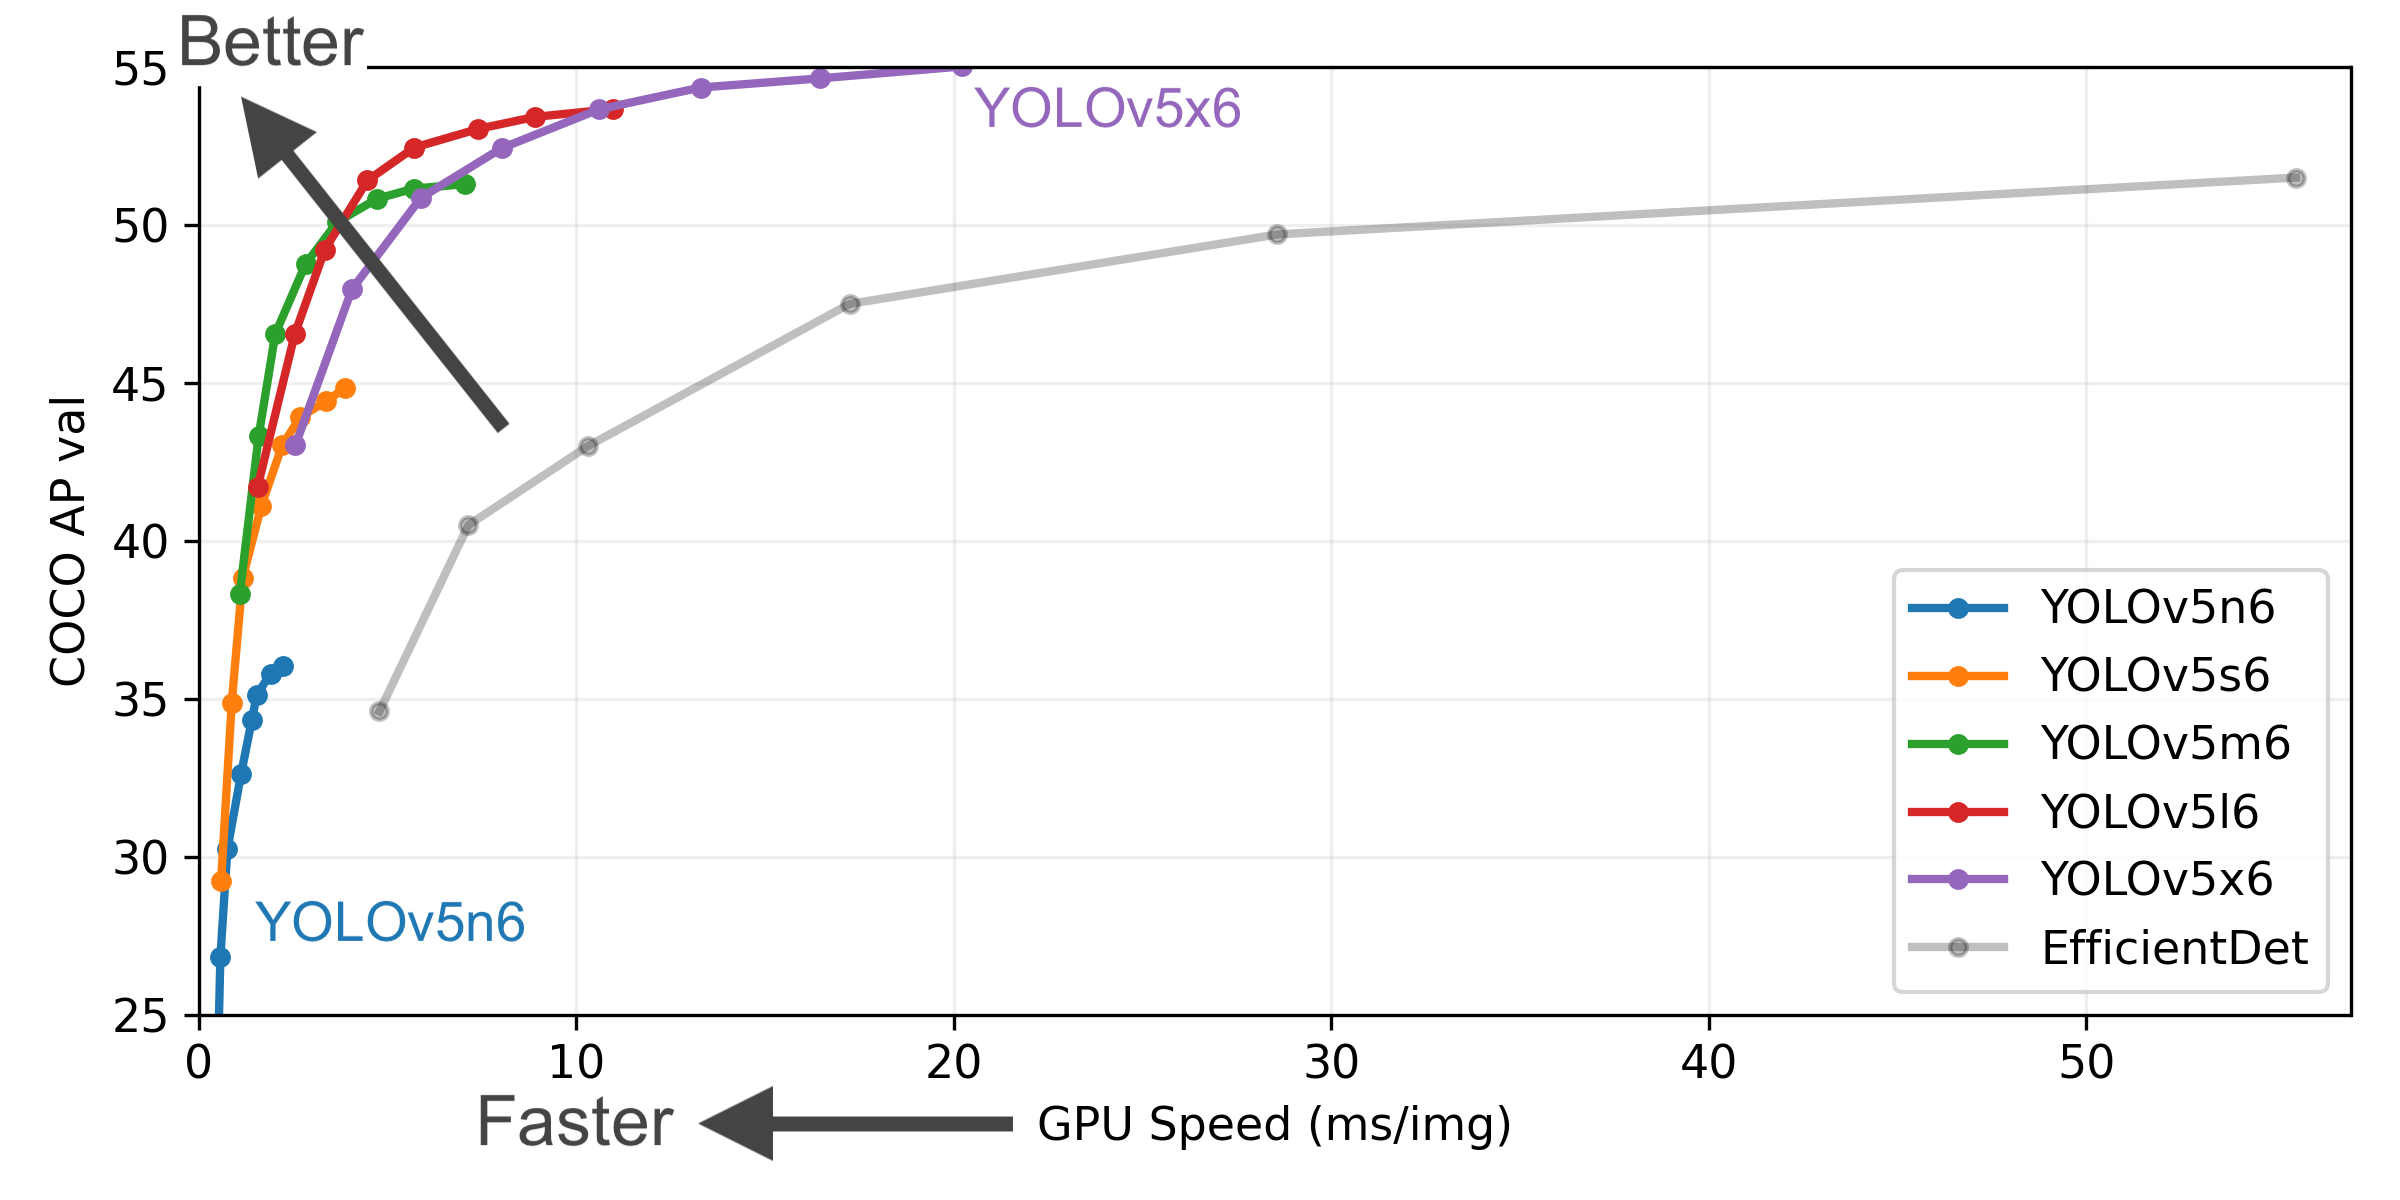
\includegraphics[width=\columnwidth]{images/yolov5-sizes.png}
    \end{center}

	\caption{Performance and speed comparison for the YOLOv5-v6.0 family of models considering the mAP@0.5:0.95 metric measured on the 5000-image COCO val2017 \cite{lin2014microsoft} dataset. The plot shows the performance of different models varying the input size of the image from $256 \times 256$px to $1536 \times 1536$px \cite{glenn_jocher_2021_5563715}.}
	\label{fig:yolo-sizes}%
\end{figure}


\begin{table}
    \centering
    \centerline{\begin{tabular}{c|c|c|c|c|c|c|c}
        \hline
        \multirow{2}{*}{ \textbf{Model}} & 
        \textbf{size} &
        \textbf{$\text{mAP}^{\text{val}}$} & 
        \textbf{$\text{mAP}^{\text{val}}$} & 
        \textbf{Speed} & 
        \textbf{Speed} & 
        \textbf{\# params} & 
        \textbf{FLOPs} \\
        & (pixels) & \textbf{0.5:0.95} & \textbf{0.5} & \textbf{CPU} (ms) & \textbf{GPU} (ms) & (M) & @640px (B) \\
        \hline
        YOLOv5n & 640 & 28.0 & 45.7 & 45 & 6.3 & 1.9 & 4.5 \\
        YOLOv5s & 640 & 37.4 & 56.8 & 98 & 6.4 & 7.2 & 16.5 \\
        YOLOv5m & 640 & 45.4 & 64.1 & 224 & 8.2 &  21.2 & 49.0 \\
        YOLOv5l & 640 & 49.0 & 67.3 & 430 & 10.1 & 46.5 & 109.1 \\
        YOLOv5x & 640 & 50.7 & 68.9 & 766 & 12.1 & 86.7 & 205.7 \\
        \hline
        \hline
        
        YOLOv5n6 & 1280 & 36.0 & 54.4 & 153 & 8.1 & 3.2 & 4.6 \\
        YOLOv5s6 & 1280 & 44.8 & 63.7 & 385 & 8.2 & 12.6 & 16.8 \\
        YOLOv5m6 & 1280 & 51.3 & 69.3 & 887 & 11.1 &  35.7 & 50.0 \\
        YOLOv5l6 & 1280 & 53.7 & 71.3 & 1784 & 15.8 & 76.8 & 111.4 \\
        YOLOv5x6 & 1280 & 55.0 & 72.7 & 3136 & 26.2 & 140.7 & 209.8 \\
        \hline        
        \end{tabular}}
    \caption{Performance comparison considering the mAP@0.5:0.95 metric of all checkpoints of YOLOv5-v6.0 trained for 300 epochs on COCO dataset \cite{glenn_jocher_2021_5563715}.}
    \label{table:yolo-sizes}
\end{table}

The class-agnostic logo detector is based on YOLOv5m6, shown in \autoref{table:yolo-sizes}, with image input size set to $512 \times 512$px and pretrained on the COCO dataset. The model is then finetuned for 30 epochs on the task of class-agnostic logo recognition, thus, not distinguishing the specific logo class. 

\section{Classification}
\label{sec:method-classifier}
Given the ROIs, the classification of each cropped region is performed by a model trained using CIL techniques. To achieve this goal, the classifier is trained using the DER algorithm \cite{yan2021dynamically} described in \autoref{sec:der-algorithm}.

\subsection{ResNet-34}
The DER algorithm introduces a new feature extractor $\mathcal{F}_t$ at each incremental step. This feature extractor consists of a Convolutional Neural Network (CNN). In the developed system, the backbone of the CNN used as feature extractor is ResNet-34 \cite{he2016deep} pre-trained on ImageNet1000 \cite{deng2009imagenet}.

The peculiar aspect of the ResNet architecture are the Residual Connections, shown in \autoref{fig:residual-connection}.. These connections are a type of skip-connection that, instead of learning unreferenced functions, learn residual functions with respect to the layer inputs. Formally, denoting the desired underlying mapping as $\mathcal{H}(x)$, we let the stacked nonlinear layers fit another mapping of $\mathcal{F}(x) := \mathcal{H}(x) - x$. The original mapping is recast into $\mathcal{F}(x) + x$. 

The intuition is that it is easier to optimize the residual mapping than to optimize the original, unreferenced mapping. To the extreme, if an identity mapping were optimal, it would be easier to push the residual to zero than to fit an identity mapping by a stack of nonlinear layers \cite{he2016deep}.

The architecture of ResNet-34, shown in \autoref{table:resnet}, consists in multiple stacked building blocks. Each building block, represented by the brackets in \autoref{table:resnet}, adopt the residual connection described above. The total number of parameters of ResNet-34 used as feature extractor at each incremental step is 23 million.

\begin{table}
    \centering
    \begingroup
    
    \begin{tabular}{>{\centering\arraybackslash}p{.3\textwidth}|>{\centering\arraybackslash}p{.3\textwidth}|>{\centering\arraybackslash}p{.3\textwidth}}


        \hline
        \multicolumn{3}{c}{\textbf{ResNet-34 architecture}}\\
        \hline
        \textbf{Layer name} & \textbf{Output size} & \textbf{Layer} \\
        \hline
        \hline
        conv1 & $112 \times 122$ & $7 \times 7, 64,$ stride $2$ \\
        \hline
          & $56 \times 56$ & $3 \times 3$ max pool, stride $2$ \\
        \hline

        \[ \textrm{conv2\char`_x} \] &  \[56 \times 56 \] & \[\left[ \begin{array}{c} 3 \times 3, \, 64\\ 3 \times 3, \, 64  \end{array}\right] \times 3 \]\\
        \hline

        \[ \textrm{conv3\char`_x} \] &  \[28 \times 28 \] & \[\left[ \begin{array}{c} 3 \times 3, \, 128\\ 3 \times 3, \, 128  \end{array}\right] \times 4 \]\\
        \hline

        \[ \textrm{conv4\char`_x} \] &  \[14 \times 14 \] & \[\left[ \begin{array}{c} 3 \times 3, \, 256\\ 3 \times 3, \, 256  \end{array}\right] \times 6 \]\\
        \hline

        \[ \textrm{conv5\char`_x} \] &  \[7 \times 7 \] & \[\left[ \begin{array}{c} 3 \times 3, \, 512\\ 3 \times 3, \, 512  \end{array}\right] \times 3 \]\\
        \hline
        & $1000 \times 1$ & average pool \\
        \hline
        FC & $1000 \times 1$ & $1000$-d FC layer, softmax \\
        \hline
        \end{tabular}
    \endgroup
    \caption{Architecture of ResNet-34, the brackets represent}
    \label{table:resnet}
\end{table}

\begin{figure}%
	\centering
	\subfloat[\centering Residual learning: a building block]{{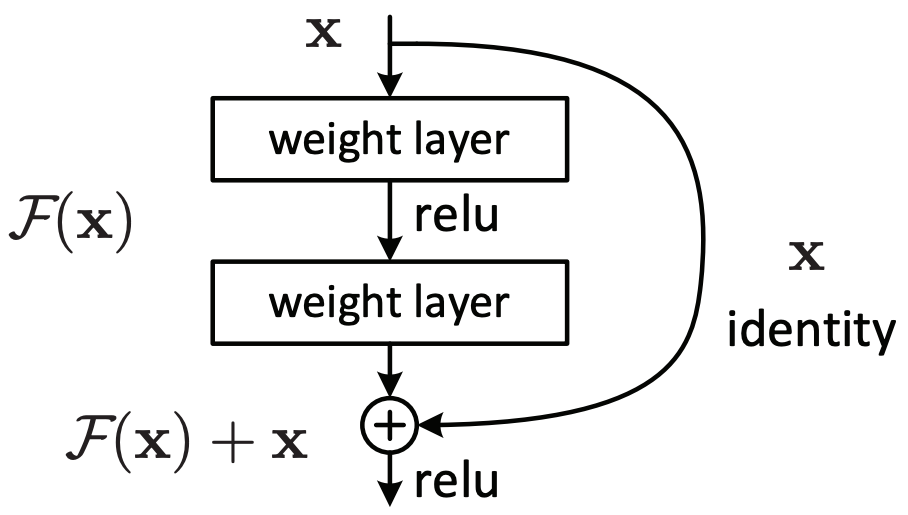
\includegraphics[width=0.45\textwidth]{images/residual-theory.png} }}%
	\hfill
	\subfloat[ An example of residual connection in a building block on a $56 \times 56$ feature maps. This building block corresponds to \textrm{conv2\char`_x} in \autoref{table:resnet} ]{{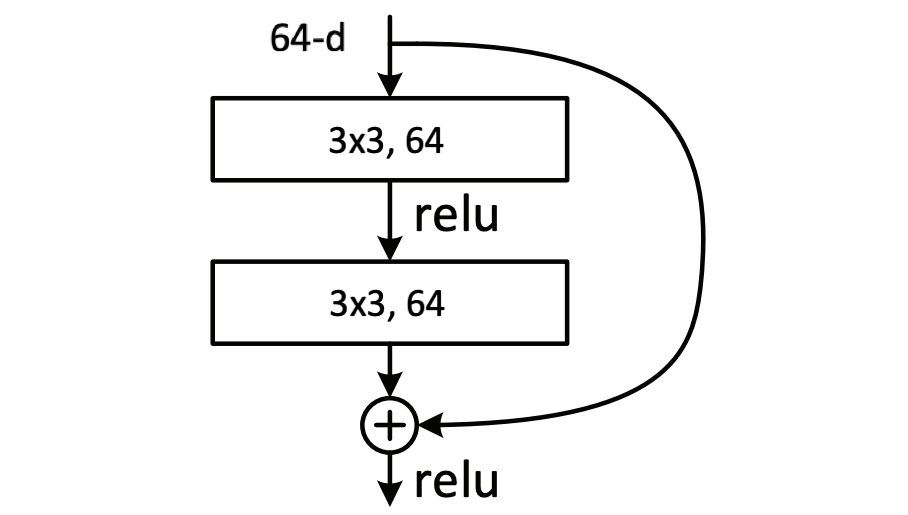
\includegraphics[width=0.45\textwidth]{images/residual-practice.png} }}%
	\caption{Residual connection in ResNet architecture \cite{he2016deep}.}%
	\label{fig:residual-connection}%
\end{figure}

\subsection{CIL classifier}
The classifier is developed in a CIL setup. In this way it is possible to recognize new logos by enriching the old knowledge. The algorithm used for CIL is the DER algorithm described in \autoref{sec:der-algorithm}. An implementation of the DER algorithm is given by PyCIL\footnote{PyCIL GitHub repository: \href{https://github.com/G-U-N/PyCIL}{https://github.com/G-U-N/PyCIL}}, and has been used as the starting for the development of the CIL classifier. All the changes performed to the implementation of DER in PyCIL are described in the following sections, and can be found in this\footnote{GitHub repository relative to the CIL model of this thesis: \\ \href{https://github.com/gianlucagiudice/PyCIL}{https://github.com/gianlucagiudice/PyCIL}} GitHub repository.


The implementation of DER in PyCIL reflects the description of the DER paper, the only change is relative to the third stage of the DER algorithm referred to as "Classifier Learning Stage" in \autoref{sec:der-algorithm}. In fact, in PyCIL the Classifier Learning Stage is performed using the WA described in \autoref{sec:wa-biased}; in this way it is possible to solve the problem of biased weights in the FC layer without the need to train the model further. It is important to point out that although this step of the original algorithm has been changed, the final performance reported by PyCIL is very similar to that obtained from the original DER paper (see \autoref{table:cil-results}).

\subsection{Regularization techniques}
In order to prevent the overfitting of the model on the test set images, the architecture of the Neural Network (NN) created using the DER algorithm has been changed. Starting from the original architecture shown in \autoref{fig:der-pipeline}, a dropout layer has been added before the FC layer represented in the figure by the classifier $\mathcal{H}_t$.

\subsubsection{Dropout}
DNN with a large number of parameters are prone to overfitting the training data and do not generalize well on the test set.
Dropout \cite{srivastava2014dropout} is a technique for addressing this problem.

At training time, the units of the NN, along with their connections, are randomly dropped with a specified probability $p$ (a common value is $p = 0.5$). At test time, all units are present, but with weights scaled by $p$ (i.e. $w$ becomes $pw$). This procedure is shown in \autoref{fig:dropout}.

The idea is to prevent co-adaptation, where the NN becomes too reliant on particular connections, as this could be symptomatic of overfitting. Intuitively, dropout can be thought of as creating an implicit ensemble of NN.

\begin{figure}%
	\centering
	\subfloat[\centering Standard neural network]{{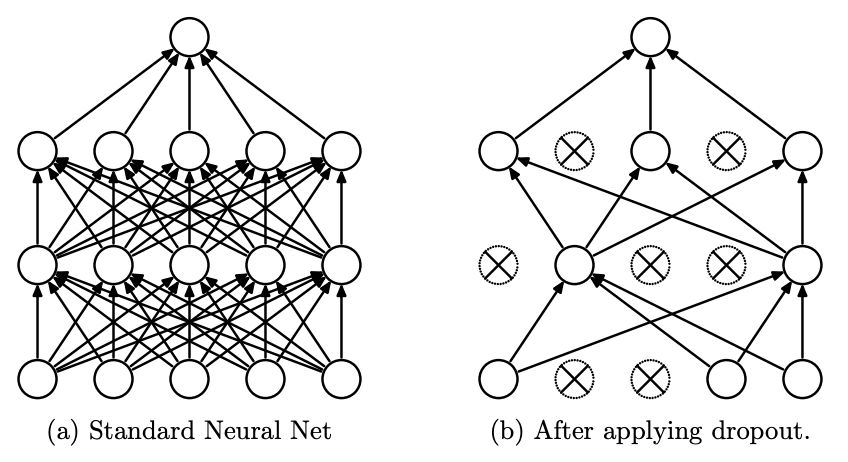
\includegraphics[width=0.30\textwidth,trim={0 24 220 0},clip]{images/dropout.png} }}%
	\hspace*{2cm}
	\subfloat[\centering Neural network after applying dropout ]{{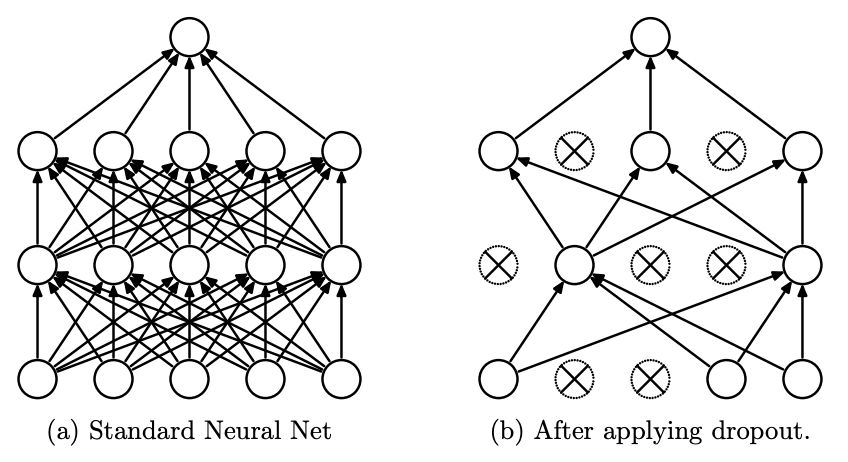
\includegraphics[width=0.30\textwidth,trim={220 24 0 0},clip]{images/dropout.png} }}%
	\caption{Dropout mechanism in a Neural Network with 2 hidden layers \cite{srivastava2014dropout}.}%
	\label{fig:dropout}%
\end{figure}

\subsection{Data Augmentation}
As discussed in \autoref{sec:dataset-stat}.
\subsection{Training}
trained on this machine with this gpu.
\subsubsection{Early stopping}
\subsubsection{SGD and Adam optimizer}
wieght decay

\subsection{Pruning}
in order to reduce the number of parameter has been implemented the amsking and pruning described in section.
\label{sec:method-pruning}
\section{Knowledge distillation}

\label{sec:method-kd}
\section{Proposed baseline for the classifier}
\label{sec:method-baseline}
\subsection{Baseline without incremental steps}
\subsection{ResNet-152 architecture}
\subsection{DER-based architecture}